\documentclass{beamer}
\usepackage{amsmath}
\usepackage{enumitem}
\usepackage{tikz}
\usepackage{url}

% put bullets back in font package
\setlist[itemize,1]{label={\fontfamily{cmr}\fontencoding{T1}\selectfont\textbullet}}

% remove stupid navigation tools and add page numbers
\mode<presentation>{\usetheme{Malmoe}}
\setbeamertemplate{navigation symbols}{}

\addtobeamertemplate{navigation symbols}{}{%
    \setbeamercolor{footline}{fg=black}
    \usebeamerfont{footline}%
    \usebeamercolor[fg]{footline}%
    \hspace{1em}%
    \insertframenumber/\inserttotalframenumber
}

\newcommand{\ignore}[1]{}
\newcommand*{\diff}{\mathsf{d}}
\newcommand{\some}{{\color{red} something}}
\renewcommand{\vec}[1]{\mathbf{#1}}

\newcounter{mybox}
\newcommand\tikzmark[1]{%
\tikz[remember picture,overlay] \node[inner xsep=0pt] (#1) {};
}
\newcommand\ColorBox[2][]{%
\stepcounter{mybox}%
\node[draw=blue,fill=blue!20,align=left,#1] (box\themybox) {#2};
}

\title[Free energy of a liquid]{Free energy of a liquid: separation, characterization, and why anyone cares}
\author{Brenden Vischer}
 
\usebackgroundtemplate%
{%
  \tikz\node[opacity=.1] {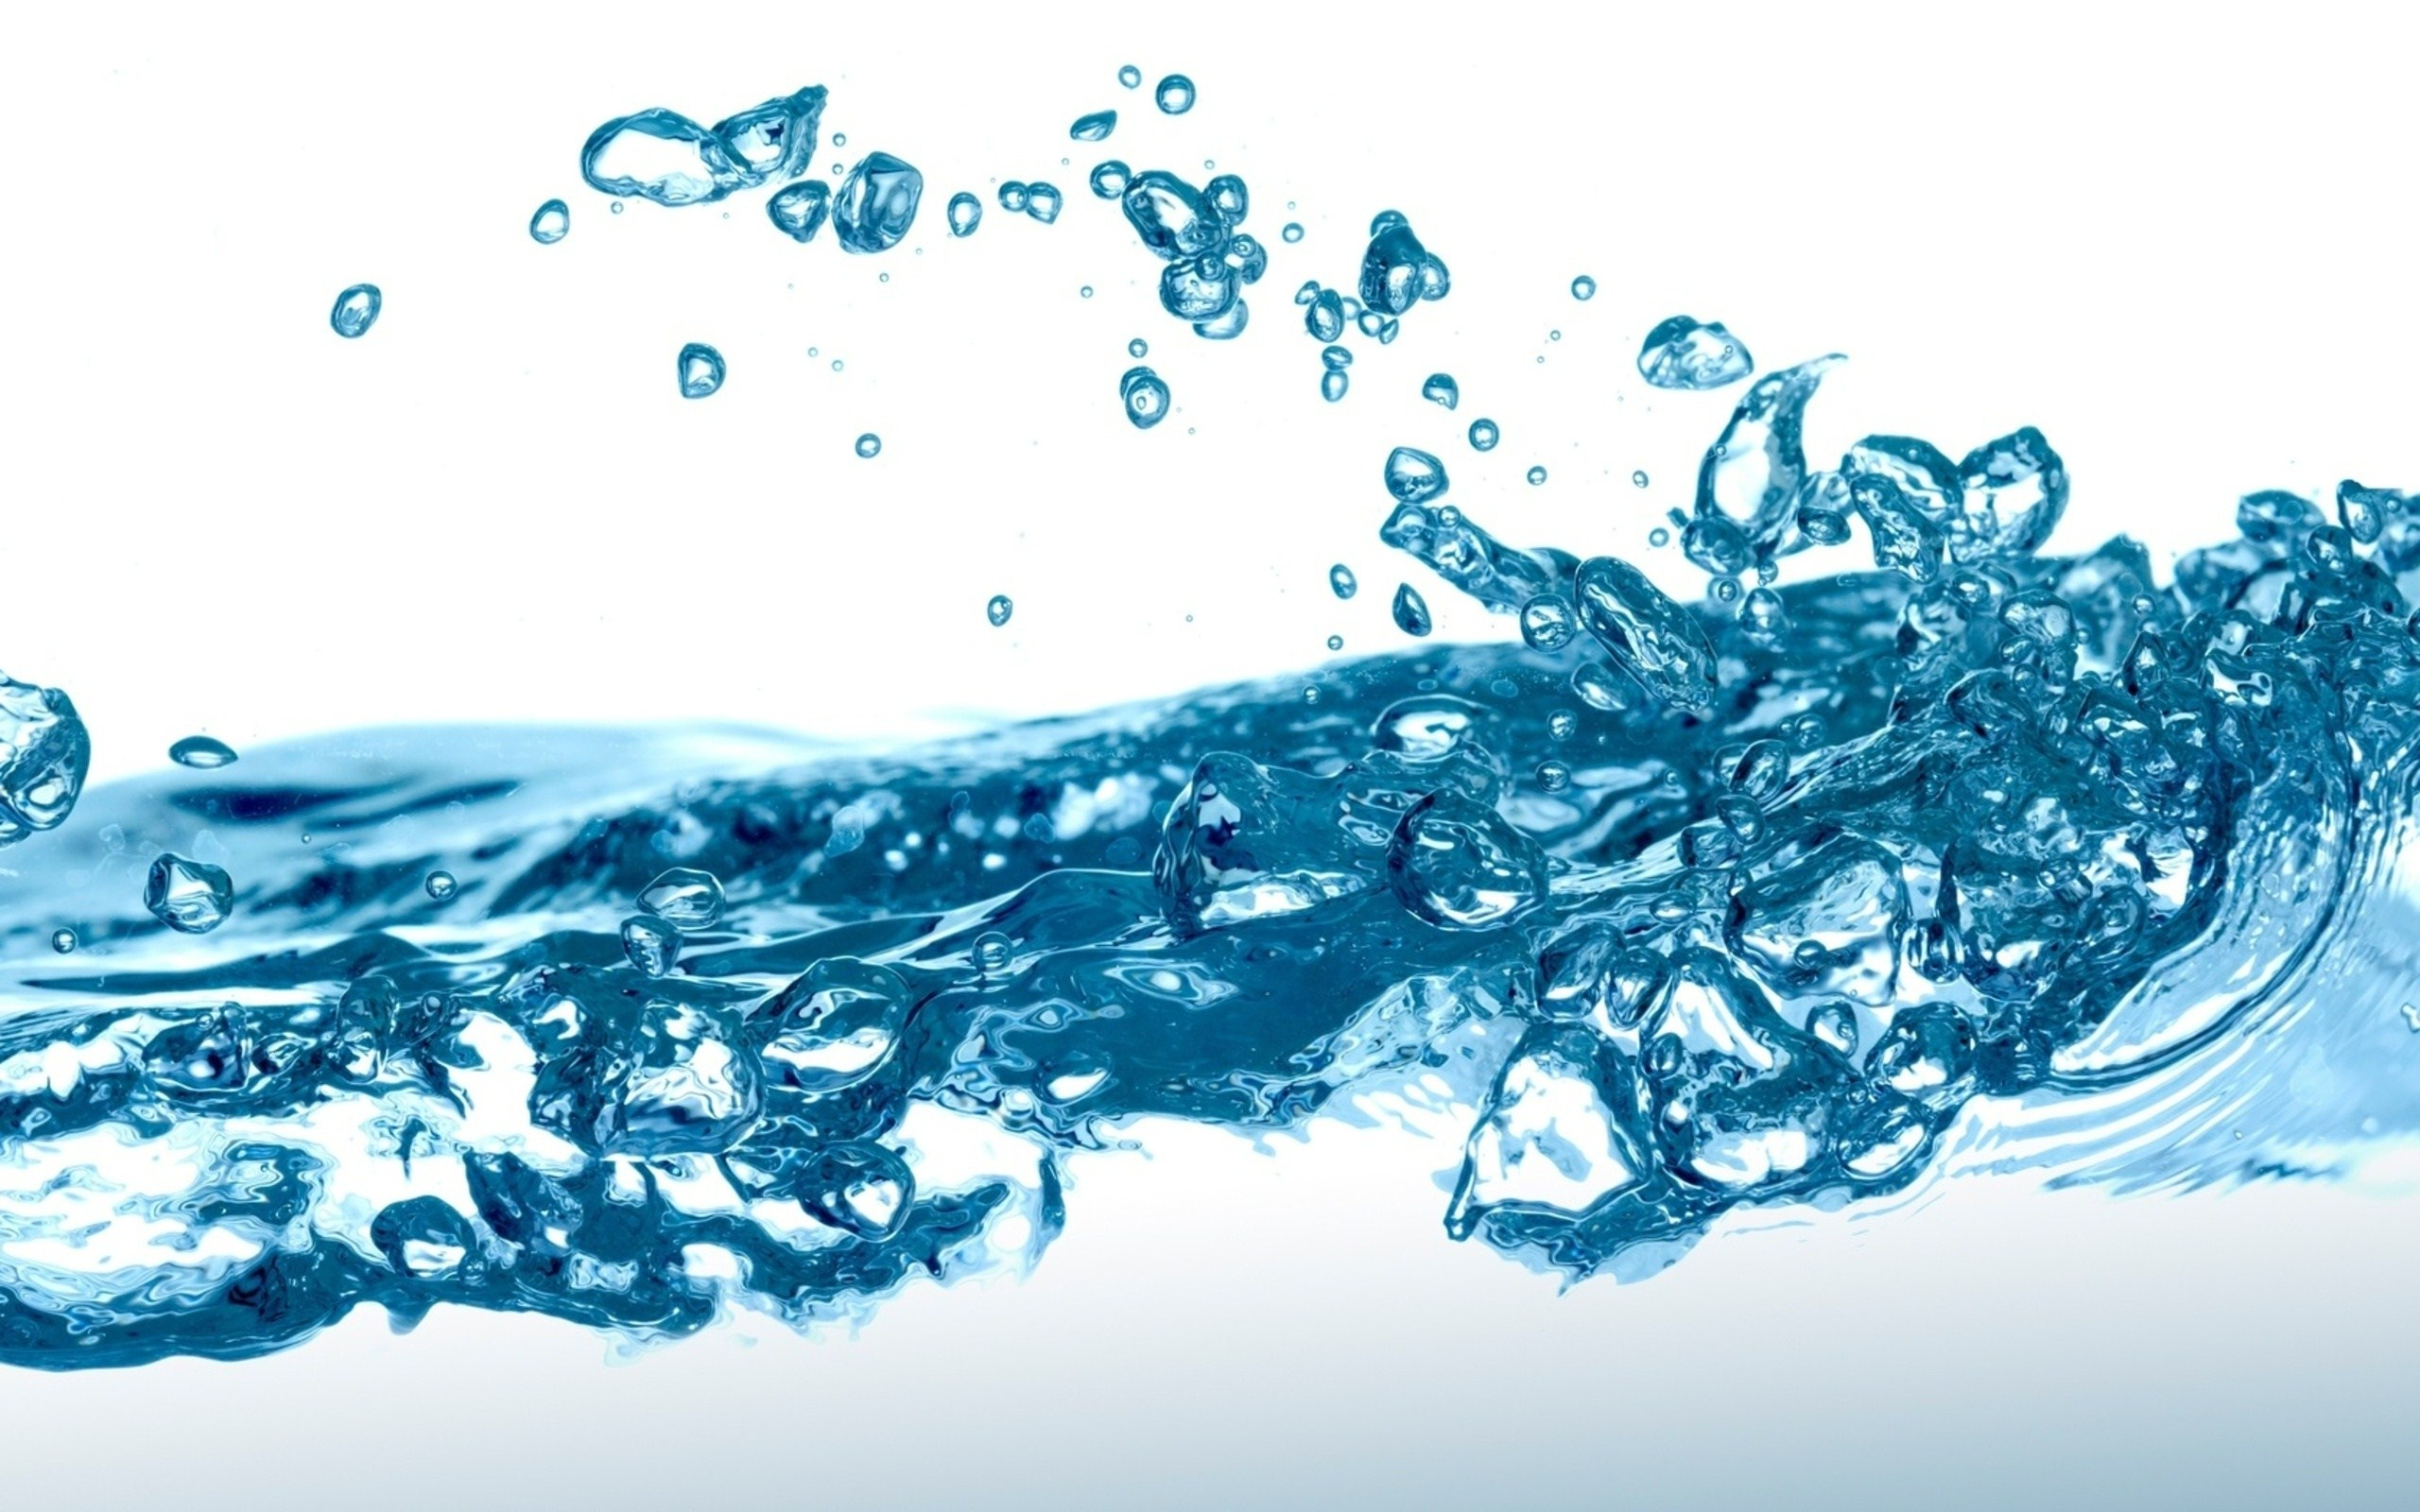
\includegraphics[width=\paperwidth,height=\paperheight]{figs/background.jpg}};%
}

\setlength\intextsep{-2em}

%%% DOCUMENT %%%

\begin{document}
\setbeamercolor{whitebox}{bg=gray!40}

%%main

\begin{frame}
	\titlepage
\end{frame}

%% Body
\AtBeginSection[]
{\begin{frame}{Table of Contents}
	\tableofcontents[currentsection]
\end{frame}}

\section*{Introduction}
\subsection*{The liquid phase}
\begin{frame}{The liquid phase}
	\begin{columns}[T]
		\column{.5\textwidth}
		\begin{figure}
			\frame{\includegraphics[width =\textwidth]{figs/phase-new}}
			\caption{Phase diagram for an arbitrary compound.}
		\end{figure}
		\column{.5\textwidth}
		\begin{block}{Phases}
			\begin{itemize}
				\item Solid: energy dominates
				\item Gas: entropy dominates
				\item Liquid: both
			\end{itemize}
		\end{block}
		\begin{block}{Liquids}
			\begin{itemize}
				\item Short range repulsion and long range attraction 
			\end{itemize}
		\end{block}
	\end{columns}
	
\end{frame}

\subsection*{Why care about liquids?}
\begin{frame}{Why care about liquids?}
		\begin{columns}[t, onlytextwidth]
			\column{.5\textwidth}
			\begin{figure}
				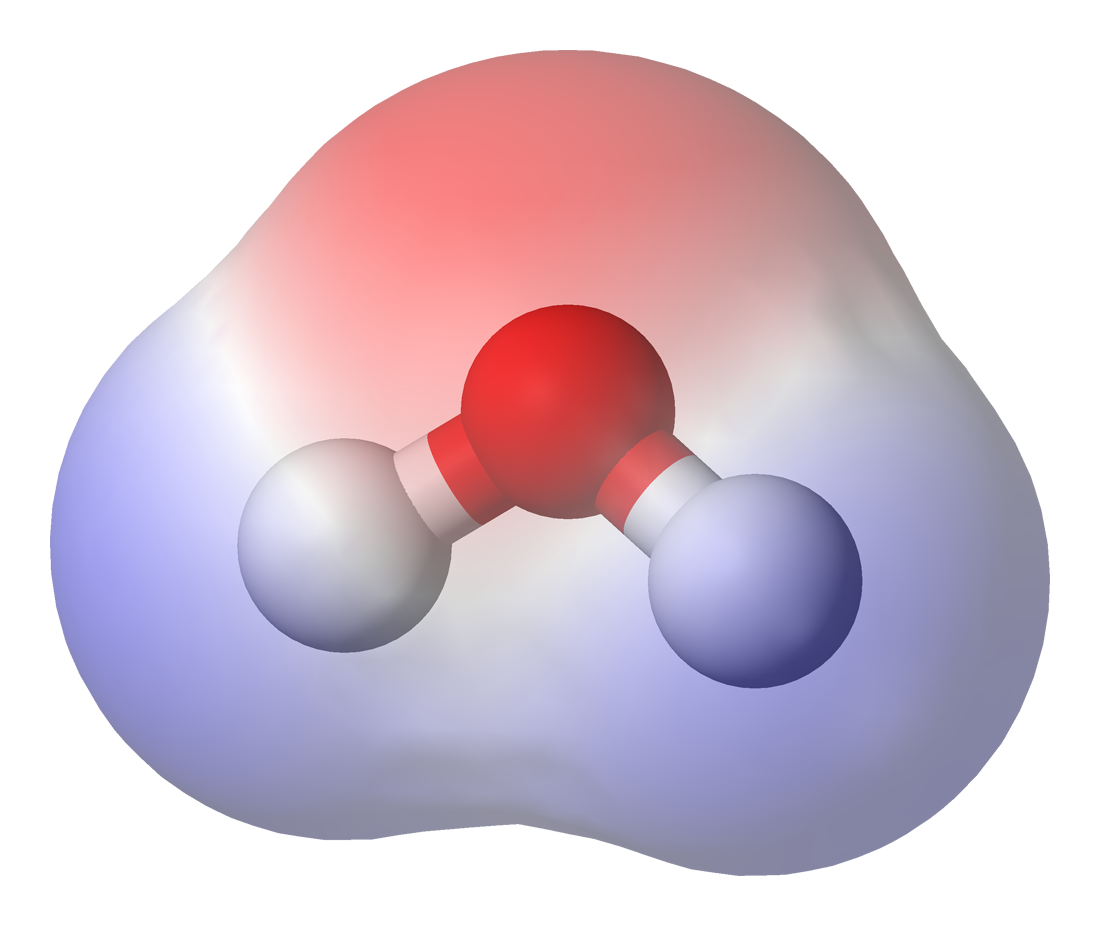
\includegraphics[width=\textwidth]{figs/water.png}	
			\end{figure}
			\column{.5\textwidth}
			\begin{block}{Water!}
			\begin{itemize}
				\item $\approx 70\%$ of Earth surface and your weight
				\item Seems simple, but is complicated
				\item Still poorly understood 
			\end{itemize}
			\end{block}
			\begin{block}{Free energy of water}
			 	% seg is HS + dispersion (SW/LJ), chain is covalent bonds, assoc is hydrogen bonds
				\begin{align*}
					F_{\text{water}} &= F_{id} + F_{HS} + F_{attr} + F_{assoc} 
				\end{align*}
			\end{block}
		\end{columns}
\end{frame}

\subsection*{What is free energy?}
\begin{frame}{What is free energy?}
		\begin{block}{Intuitive}
			$F$ - the available work in the system
		\end{block}
		\begin{block}{Mathematics}
		\vspace{1em}
		\begin{columns}[t]
		\column{.5\textwidth}		
		{\centering Thermodynamics:
		\begin{align*}
			\diff F &= - S\,  \diff T + P\, \diff V
		\end{align*}}
		\column{.5\textwidth}
		{\centering
		Statistical Mechanics
		\begin{align*}
		F &= - k_B T \ln Z
		\end{align*}}
		\end{columns}
		\end{block}		
		Why Helmholtz and not Gibbs?
	\begin{itemize}
		\item Control temperature and volume 
		\item Entropy a more preferable partial derivative
	\end{itemize}
	\end{frame}

\section*{Separation and characterization}
\subsection*{Separation}
\begin{frame}{Separation}
	%\begin{itemize}
	%\setlength\itemsep{-2em}
	%	\item 
			\begin{align*} 
				Z &= \sum_i^{\text{\tiny States}} e^{-\beta E_i}\,, & E_i &= \Phi_i(\mathbf{r}_1,\, \dots,\, \mathbf{r}_N) + \sum_j^N K_j(\mathbf{p}_j)
			\end{align*}
	%	\item %Since $E = K + V$, with $N$ particles: 
			\begin{align*}
    		Z = \frac{1}{N!}\int_{s_1} \cdots \int_{s_N} \diff\mathbf{r}_1~ \diff\mathbf{p}_1\cdots ~\diff\mathbf{r}_N~ \diff\mathbf{p}_N ~e^{-\beta \Big[\Phi(\mathbf{r}_1,\, \dots,\, \mathbf{r}_N) + K(\mathbf{p}_1) + \cdots + K(\mathbf{p}_N))\Big]}\\
			\end{align*}
	%	\item %which simplifies to 
			\begin{align*}
			Z &= \boxed{\frac{1}{ N!} \tikzmark{a}\left[V\int_s \,\diff\mathbf{p}~e^{-\beta K(\mathbf{p})}\right]^{N}} \,\cdot\, \boxed{ \int_s \frac{\diff\mathbf{r}^N}{V^N}\tikzmark{b} ~e^{-\beta \Phi(\mathbf{r_1},\, \dots,\, \mathbf{r_N})}} 
			\end{align*}
		%\item %Let's call them 
		%	\begin{align*}
		%		Z &= Z_{id}(\mathbf{p})\,Z_{exc}(\mathbf{r_1},\, \dots\, ,\mathbf{r_N})	
		%	\end{align*}
	%	\end{itemize}	
	\begin{tikzpicture}[remember picture,overlay]
		\ColorBox[xshift=2cm]{Ideal}
		\draw[blue,->] (box1) -| ([xshift=10pt]a.south west);
		\ColorBox[xshift=10cm,fill=blue!20,draw=blue]{Excess}
		\draw[blue,->] (box2) -| ([xshift=10pt]b.south west);
	\end{tikzpicture}
	%\vspace{1em}
		\begin{align*}
			F &= F_{id} + F_{exc} 	
		\end{align*}
\end{frame}

\subsection*{Characterization}
% \subsubsection*{Ideal}
% \begin{frame}{Ideal gas free energy}
% 	%\begin{columns}[t, onlytextwidth]
% 	%	\column{.5\textwidth}
% 			%\begin{itemize}
% 			%	\item 
% 				\begin{align*}
% 					Z_{id} &= \frac{1}{N!}\left(V\int \,\diff\mathbf{p}~e^{-\beta K(\mathbf{p})}\right)^{N}	 	
% 				\end{align*}
% 				\begin{align*}
% 					\mathbf{p} &= \hbar \mathbf{k} = \hbar\left( \frac{2\pi}{V^{1/3}}n_x \hat x + n_y \hat y + n_z \hat z\right)
% 				\end{align*}
% 				\begin{align*}
% 					Z_{id} = \frac{(2\pi\hbar)^{3N}}{V^N N!}&\Big[V \int_0^\infty \diff^3 n ~e^{ \frac{-2\beta \hbar^2\pi^2}{mL^2}(n_x^2 + n_y^2 + n_z^2)}\Big]^{N} 	
% 				\end{align*} 
				 
% 				\begin{align*}
%     				Z_{id} &= \left(\frac{h^{3N} V^N}{N!\Lambda^{3N}}\right) \,, & \Lambda &= \frac{\hbar\sqrt{2\pi}}{\sqrt{m k_B T}}
% 				\end{align*}
% 			%\end{itemize}
% 		%\column{.5\textwidth}
% 		%	\begin{figure}
%  		%		\includegraphics[width=\textwidth]{ideal-F-vs-T.pdf}
%  		%		\caption{\tiny Free energy of the ideal gas}
%  		%		\label{ideal}
%  		%	\end{figure}
% 	%\end{columns}
% \end{frame}

\subsubsection*{Excess}
\begin{frame}{Excess free energy}	
	\begin{columns}[t]
	\setlength\abovedisplayskip{-2pt} 
	\column{.4\textwidth}	
	\begin{align*}
		Z_{exc} &= \int_s \frac{\diff\mathbf{r}^N}{V^N} ~e^{-\beta \Phi(\mathbf{r_1}, \mathbf{r_2}, \dots \mathbf{r_N})}
	\end{align*}
	\begin{itemize}
		\item No algebraic expression for even simple $\Phi$
		\item Need to use models, simulations to approximate behavior
		\item Even with models...
	\end{itemize}
	\column{.6\textwidth}
	\begin{figure}
		\frame{\includegraphics[width=\textwidth]{figs/phi12}}
		\caption{Hard sphere and square well intermolecular pair potentials.}
	\end{figure}
		% \begin{block}{Hard sphere fluid}
	% \setlength\abovedisplayskip{-2pt} 
	% 	\begin{equation*} 
	% 		\Phi_{12}(\mathbf r) = \begin{cases}\infty & |\vec{r}|\leq \sigma\\  0 & |\vec{r}| > \sigma \end{cases}
	% 		\label{phi12_hs}
	% 	\end{equation*}
	% \end{block}
	% \begin{block}{Square well fluid}
	% \setlength\abovedisplayskip{-2pt} 
	% 	\begin{equation*} 
	% 		\Phi_{12}(\mathbf r) = \begin{cases}\infty & |\vec{r}|\leq \sigma\\ -\epsilon & \sigma \leq |\vec{r}| \leq \sigma\lambda\\ 0 & |\vec{r}| > \sigma\lambda \end{cases}
	% 		\label{phi12_sw}
	% 	\end{equation*}
	% \end{block}
	\end{columns}
\end{frame}


\subsection*{Methods}
\begin{frame}{Methods}
	\begin{figure}
		\frame{\includegraphics[width=.7\textwidth]{figs/integration.pdf}}
	\end{figure}
	\begin{itemize}
		\item Thermodynamic Integration: integration over densities
		\item Square Well Monte Carlo: integration over temperature
	\end{itemize}
\end{frame}

\subsection*{Results}
\begin{frame}{Results}
\begin{columns}
	\column{.7\textwidth}
        FIXME the file figs/Fabs-vs-eta is missing
	%% \frame{\includegraphics[width=\textwidth]{figs/Fabs-vs-eta}}
	\column{.4\textwidth}
	\begin{itemize}
		\item Two doubling regimes simulated
		\item Becomes more negative with increasing temperature, density 
	\end{itemize}
\end{columns}
\end{frame}

\section*{Final thoughts}
\subsection*{Remarks}
\begin{frame}{Remarks}
	\begin{itemize}
		\item Liquids - however simple - are very complicated
		\item Simplest models have no analytic solutions
		\item Separation enables some behavioral investigation
	\end{itemize}
\end{frame}
\subsection*{References}
\begin{frame}{References}
	\tiny
	\begin{itemize}
		\item Retrieved from \url{https://nicokrisch.files.wordpress.com/2014/05/}
		\item Retrieved from \url{https://en.wikipedia.org/wiki/Chemical_polarity}
		\item I. M. J.-P. Hansen, Theory of Simple Liquids, $3^{\text{rd}}$ ed. (Academic Press, 2006).
		\item M. A. Perlin, ``Optimizing monte carlo simulation of the square-well fluid,'' (2015), Oregon State University.
		\item A. Valeske, ``Determining free energies of hard sphere fluids via monte carlo simulation'' (2015), Oregon State University.
	\end{itemize}
\end{frame}
% \section*{Introduction}
% \subsection*{Motivation}
% \begin{frame}{Motivation}
% \begin{itemize}
% 	\item Thermodynamic properties for bulk fluids are known, but typically only exist as ``black box'' calculations, where intermediate results are not attainable. A mechanism to investigate the intermediate calculation allows for [many important things; ``checking SAFT'', ``establishing dominant wavelengths'']  
% 	\item Idea: decompose the bulk into smaller systems with specified fluctuation wavelengths that are present in the bulk
% 	\item Calculating the energy of these constituent systems indicates how energetic that particular length scale is
% \end{itemize}
% \end{frame}



% \subsection*{Criticality}
% \begin{frame}{Self similarity and the critical point}
% 	\begin{columns}
% 		\column{.5\textwidth}
% 			\begin{itemize} \small
% 				\item The critical point is the temperature and pressure at which liquid and gas become indistinguishable; the terminating point on a phase digram (Figure~\ref{phase}) 
% 				\item All length scales present (that is, all wavelengths) in fluctuations near the critical point, so each length scale looks the same - ``self similarity''
% 				\item Each wavelength is independent, so we can investigate each independently - but how?
% 			\end{itemize}
	
% 		\column{.5\textwidth}
% 			\begin{figure}
% 				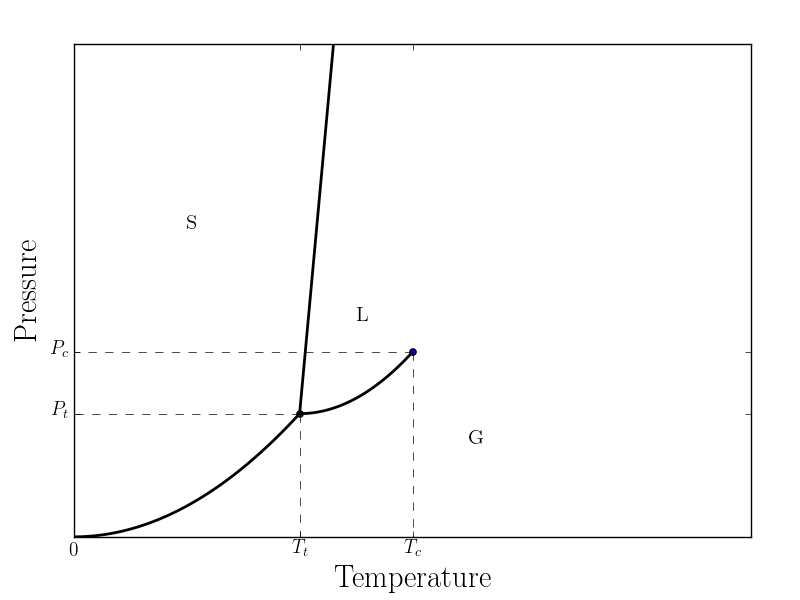
\includegraphics[width=\textwidth]{phase.png}
% 				\caption{\tiny Phase diagram of an arbitrary fluid. Labeled are the temperatures and pressures at which all three phases are present (triple point) and the critical point}
% 				\label{phase}
% 			\end{figure}
% 	\end{columns}
% \end{frame}

% \subsection*{Energy}
% 	\begin{frame}{Free energy and the burden of calculation}
% 		\begin{itemize}
% 			\item Stuff
% 		\end{itemize}
% 	\end{frame}

\end{document}
